\chapter{Feedback Control Design}
\label{chp:controller}

\section{Balancing Controller}
% WHAT you are going to present in this chapter/section
% WHY you are presenting it, and
% HOW you are going to present it

Provided the robotic gymnast is in the vicinity of the unstable equilibrium position, a balancing controller is required to balance the system. The design approach is based on the premise that the swing-up controller will swing the robotic gymnast to the vicinity of the unstable equilibrium position where the balancing controller will take over. This section will focus on aspects required to implement this balancing controller.\\


\subsection{Controller Architecture}

\begin{figure}
	\centering
	% System Combination
% Harish K Krishnamurthy <www.ece.neu.edu/~hkashyap/>
\documentclass{article}

\usepackage{tikz}
\usetikzlibrary{shapes,arrows,shadows}
\usepackage{amsmath,bm,times}
\newcommand{\mx}[1]{\mathbf{\bm{#1}}} % Matrix command
\newcommand{\vc}[1]{\mathbf{\bm{#1}}} % Vector command

\begin{document}
	% Define the layers to draw the diagram
	\pgfdeclarelayer{background}
	\pgfdeclarelayer{foreground}
	\pgfsetlayers{background,main,foreground}
	
	% Define block styles used later
	
	\tikzstyle{sensor}=[draw, fill=blue!20, text width=5em, 
	text centered, minimum height=2.5em,drop shadow]
	\tikzstyle{ann} = [above, text width=5em, text centered]
	\tikzstyle{wa} = [sensor, text width=10em, fill=red!20, 
	minimum height=6em, rounded corners, drop shadow]
	\tikzstyle{sc} = [sensor, text width=13em, fill=red!20, 
	minimum height=10em, rounded corners, drop shadow]
	
	% Define distances for bordering
	\def\blockdist{2.3}
	\def\edgedist{2.5}
	
	\begin{tikzpicture}
	\node (wa) [sensor]  {$\boldsymbol{\dot{x}}= \boldsymbol{A}\boldsymbol{x}+\boldsymbol{B}$};
	\path (wa.south)+(0,-1) node (feedback) [sensor] {$u = -\boldsymbol{K}\boldsymbol{x}$};
	
	\path (wa.east)+(\blockdist/1.5,0) node (C) [sensor] {$\boldsymbol{C}$};
	\path (C.east)+(\blockdist/1.5,0) node (Y) [sensor] {$\boldsymbol{y}$};
	
	
	\path [draw, ->,thick] (wa.east) -- node [above] {} 
	(C.west);
	
	\path [draw, ->,thick] (C.south) |- node [above] {} 
	(feedback.east);
	
	\path [draw, ->,thick] (C.east) -- (Y.west);
	
	\path [draw, ->,thick] (feedback.west) -| ([xshift=-1cm]wa.west) -- (wa.west) {};
	
	%\path [draw, ->,] (C.east) -- node [above] {} 
	%	(Y.west);
	
	%\path (wa.south) +(0,-\blockdist) node (asrs) {System Combination - Training};
	
	%\begin{pgfonlayer}{background}
	%   \path (asr1.west |- asr1.north)+(-0.5,0.3) node (a) {};
	%  \path (wa.south -| wa.east)+(+0.5,-0.3) node (b) {};
	% \path (C.east |- asrs.east)+(+0.5,-0.5) node (c) {};
	
	%\path[fill=yellow!20,rounded corners, draw=black!50, dashed]
	%   (a) rectangle (c);           
	% \path (asr1.north west)+(-0.2,0.2) node (a) {};
	
	%\end{pgfonlayer}
	
	\end{tikzpicture}
	
\end{document}}
	\caption{State Space Representation of the Balancing Controller}
	\label{fig:linearSys2}
\end{figure}

Figure \ref{fig:linearSys2} shows the block diagram that implements the balancing controller, and it is clear that the state space representation for the system is used. The requirement of using the state space representation is that the system must be a linear time invariant (LTI) system. The system describe in equation (\ref{eq:condense1}) and (\ref{eq:condense2}) are not linear and thus linearisation is required. How this requirement was satisfied is discussed in the following sections.\\

Another aspect of the balancing controller is that there are no reference input to instruct the controller to guide the robotic gymnast to the unstable equilibrium position. Due to the system being linearised at the unstable equilibrium position and that the swing-up controller brings the system to this linearised region the problem is effectively a initial condition problem. The unstable poles of the system can be move to become stable using feedback and results in the system to decay to the unstable equilibrium position from an initial condition around the unstable equilibrium position.


\subsection{Requirements/Specifications and Constraints}
\subsection{Plant Linearisation}

As mentioned previously, to implement the state space representation the system must be a LTI system. This is achieved by using the Taylor Series Expansion to linearise the system at the unstable equilibrium position.\\

The independent parameters, $\phi$ and $\theta$, will be condensed from now on as a vector describes as $$ \vec{q} = 
\begin{bmatrix}
\theta \\
\phi
\end{bmatrix}
$$

The system is thus linearised at 
$$ [\vec{q_{s}},\dot{\vec{q_{s}}},\ddot{\vec{q_{s}}}]^{T}=[\pi,0,0,0,0,0]$$
with the mathematical details shown in Appendix \ref{sec:linerisation}. This linearised model can than be written in the state space form to implement a feedback gain. The state space variables are chosen as $\Delta{\vec{q}}$ and $\Delta{\dot{\vec{q}}}$ which results in the state space representation as:  $$ \dot{\vec{q}} = \boldsymbol{A}\Delta{\vec{q}} + \boldsymbol{B}u $$ and $$ \vec{y} = \boldsymbol{D}\Delta{\vec{q}} + \boldsymbol{0}u $$

The poles of the system are identified by determining the eigenvalues of the $\boldsymbol{A}$ matrix. The linearised system remains a coupled system which results that the quadratic eigenvalue problem shown in equation (\ref{eq:quadratic_eigen}) was required to be solved to identify the poles of the system. The solved quadratic eigenvalue problem results in the following poles using the system parameters in Table \ref{table:system_param}.

\begin{equation} \label{eq:quadratic_eigen}
Q(\lambda) =\lambda^{2}M + \lambda C + K
\end{equation}

$$
\vec{s} = 
\begin{bmatrix}
10.5742 \\
4.9498	\\
-11.4905 \\
-5.0215 \\

\end{bmatrix}
$$

The eigenvalues of the system are all real indicating the response of the system when disturbed is an exponential function. This can be explained by realising the linearised system is modelled as a single pendulum. Once the single pendulum is disturbed from the unstable equilibrium position it would continue to rotate downwards in the same direction and not with an oscillatory response. 


\subsection{Full State Feedback Design}
The poles of the system are pairs of positive and negative real poles that indicate an unstable system. This is expected due to the system being linearised at the unstable equilibrium position. When the linearised system is at rest, any disturbance will result in a theoretically infinite growth of the state variables, but this behaviour can be controlled by introducing feedback. \\

These poles will be moved to the desired position by using the method of dominant poles. The method of dominate poles chooses a pair of the poles for the closed-loop system and select the other open-loop poles to have real parts. This allows the higher-order system response to be characterised as a second-order response \cite{textbook}. The linearised model already has 2 negative real poles which is chosen to stay the same. The real positive poles were selected based on the following specifications.\\

These specification was selected on increasing the null controllability region with a low settling time. Due the approximation of the linearised model the null controllability region may be larger than the derived sized \cite{simple_null_controllability}. 


\subsection{Simulation Response}
\begin{figure}[h]
	\centering
	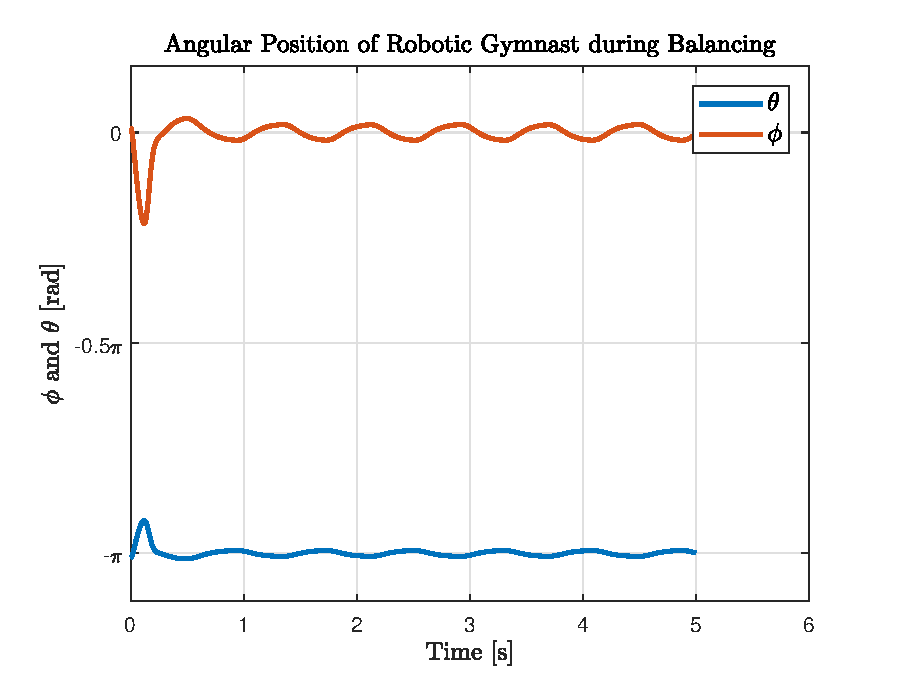
\includegraphics[scale=1]{./figs/balancing}
	\caption{Balancing of the Robotic Gymnast}
	\label{fig:balance}
\end{figure}

Figure \ref{fig:balance} shows the robotic gymnast balancing around the unstable equilibrium position with initial condition of $$ \vec{q} = 
\begin{bmatrix}
\frac{\pi}{0.1}\\
\frac{\pi}{10}
\end{bmatrix}
$$ The oscillatory response around the inverted position is due to the non-linear coulomb damping. This oscillatory response was decided to be acceptable due to assumption that the effect of coulomb damping is negligible at low velocities. This is visible in Figure \ref{fig:q1_response} where the response depart from the linear decay function near the stable equilibrium position.

The response shows that the controller meets the requirement of balancing the robotic gymnast from initial condition of $q \in []$ and reaches steady state within 1 second.





\section{Swingup Controller}
% WHAT you are going to present in this chapter/section
% WHY you are presenting it, and
% HOW you are going to present it
The swing up of the robotic gymnast is done by the non-linear feedback control system. For the robotic gymnast to swing from the stable equilibrium position to the unstable equilibrium position the feedback control must incorporate the non-linearities of the system. How these non-linearities of the system are incorporated and the design paradigm of the approach will be explained in following section.

\subsection{Controller Architecture}
\begin{figure}[h]
	\centering
	\documentclass{article}

\usepackage{tikz}
\usetikzlibrary{shapes,arrows}
\usepackage{amsmath,bm,times}
\newcommand{\mx}[1]{\mathbf{\bm{#1}}} % Matrix command
\newcommand{\vc}[1]{\mathbf{\bm{#1}}} % Vector command

\begin{document}
	\pagestyle{empty}
	
	% We need layers to draw the block diagram
	\pgfdeclarelayer{background}
	\pgfdeclarelayer{foreground}
	\pgfsetlayers{background,main,foreground}
	
	% Define a few styles and constants
	\tikzstyle{sensor}=[draw, fill=blue!20, text width=5em, 
	text centered, minimum height=2em]
	\tikzstyle{ann} = [above, text width=5em]
	\tikzstyle{block} = [sensor, text width=6em, fill=red!20, 
	minimum height=4em, rounded corners]
	\tikzstyle{sum}=[draw, fill=red!20, circle, node distance = 2cm]
	
	\tikzstyle{longblock} = [sensor, text width=10em, fill=red!20, 
	minimum height=4em, rounded corners,minimum width=6em]
	
	\def\blockdist{2.5}
	\def\edgedist{2.5}
	
	
	
	\noindent\makebox[\textwidth]{
	\begin{tikzpicture}[scale=0.8]
	% plant block
	\node (plant) [block] {Non-Linear Plant};
	
	% collocated blovk
	\path (plant)+(0,-\blockdist) node (collinear) [block] {Collocated\ Linearisation};
	
	% Annotation
%	\path (plant)+(1.5*\blockdist,0) node (output) [ann] { [ $\ddot{\theta}$ \\ $\dot{\phi}$ ] };
	
	\path (plant)+(1.2*\blockdist,0) node (output) [ann] { 
$\begin{bmatrix}
$$\ddot{\theta}$$ \\ $$\ddot{\phi}$$ 
\end{bmatrix}$
};
	
	%sumation block 1
	\path (plant)+(-\blockdist,0) node (suma1) [sum]{\Large$\Sigma$};
	
	% Non-linear control law
	\path (plant)+(-2.2*\blockdist,0) node (nonlinear) [longblock]{Non-Linear Law \ $v = K_{p}(\phi^{d}-\phi)-K_{d}\dot{\phi}$};
	
	%sumation block 2
	\path (nonlinear)+(-1.2*\blockdist,0) node (suma2) [sum]{\Large$\Sigma$};

	% Desired input
	\path (suma2)+(-1.2*\blockdist,0) node (desired) [longblock]{Desired Trajectory \ $\phi^{d} = \alpha \tan(\dot{\theta})$};

%%%%%%%%%%%%%%%%%%%%%%%%%%%%%%%%%%%%%%%%%%%%%%%%%%%%%%%%%%%%%%%%%%%%%%%%%%%%%%%%%%%%%%%%%%%%%%%%%%%%%%%%%%%%%%%%%%%%%%%%%%
	% plant to output	
%	\draw [->,thick] (plant) -- node [anchor=north east] {} + (\edgedist,0) 
%	node[right] {$[\theta$ $\phi$ $\dot{\theta}$ $\dot{\phi}$ $\ddot{\phi}$  $\ddot{\theta}]$};
	
	%plant to output
	\draw [->,thick] (plant.east) -- ([xshift=1cm]plant.east) {};
	% plant to collocated
	\draw[->,thick] ([xshift=0.5cm]plant.east) -- ([xshift=0.5cm]collinear.east) -- (collinear.east) {};
	
	% collocated lineariation to Sigma
	\draw[->,thick] (collinear.west) -| (suma1.south) {};
	
	%sigma to non-linear plant
	\draw[->,thick] (suma1.east) -- (plant.west) {};
	
	% non-linear law to sigma
	\draw[->,thick] (nonlinear.east) -- (suma1.west) {};
	
	% sigma2 to non linear
	\draw[->,thick] (suma2.east) -- (nonlinear.west) {};

	% Desired input to sigma
	\draw[->,thick] (desired.east) -- (suma2.west) {};
	
	% collocated to sigm2
	\draw[->,thick] (collinear.west) -| (suma2.south) {};
	






	% Now it's time to draw the colored IMU and INS rectangles.
	% To draw them behind the blocks we use pgf layers. This way we  
	% can use the above block coordinates to place the backgrounds   
	\begin{pgfonlayer}{background}
	% Compute a few helper coordinates
%	\path (gyros.west |- naveq.north)+(-0.5,0.3) node (a) {};
%	\path (INS.south -| naveq.east)+(+0.3,-0.2) node (b) {};
	%\path[fill=yellow!20,rounded corners, draw=black!50, dashed]
	%(a) rectangle (b);
%	\path (gyros.north west)+(-0.2,0.2) node (a) {};
	%\path (IMU.south -| gyros.east)+(+0.2,-0.2) node (b) {};
%	\path[fill=blue!10,rounded corners, draw=black!50, dashed]
%	(a) rectangle (b);
	\end{pgfonlayer}

\end{tikzpicture}
}
	
\end{document}
	\caption{Block Diagram of the Non-Linear Controller}
	\label{fig:nonlinear_controller_arch}
\end{figure}

Figure \ref{fig:nonlinear_controller_arch} shows a high-level block diagram of the multiple parts of the swing-up controller. These parts are required to work in unison to allow the robotic gymnast to swing.\\

The collocated linearisation block is the foundation on which the entire controller is built. It creates a linear response from one of the outputs of the plant. The linear response of one the outputs can than be used to follow a desired trajectory. The swing-up controller than contains a classical control theory approach where gains are selected to characterise the response of the system based on the error of the desired and actual trajectory.\\

Each of the blocks shown in the block diagram will be discussed in the section below.


\subsection{Requirements/Specifications and Constraints}
% WHAT you are going to present in this chapter/section
% WHY you are presenting it, and
% HOW you are going to present it
The requirements of the swing-up controller is to swing the robotic gymnast up under 30 seconds to the unstable equilibrium positions. In the vicinity of the unstable equilibrium position the when the non-actuated pendulum is upright $\theta = \SI{2\pi}{\radian} \pm \frac{\pi}{30}$ the controller must position the actuated pendulum between $\phi \in [-5^{\circ},5^{\circ}]$.\\

The first requirement is set to provide a feasible solution to the swing-up of the robotic gymnast and allow the swing-up sequence to be captivating. The second requirement is set to ensure the linear approximation holds when the balancing controller is active to bring the system to the unstable equilibrium position and balance.

Constraints that is placed on the controller is the stall torque of the motor. 

\subsection{Feedback Linearisation}
It has been shown that it is not possible to linearise the dynamics of the gymnast by means of static state feedback and non-linear transformation \cite{murray}, but it is possible to achieve a linear response from one of the outputs of the plant by implementing a non-linear feedback. This non-linear feedback is the partial feedback linearisation.\\

Collocated linearisation is a form of partial feedback linearisation where a non-linear control input $\tau$ is used to linearise the response of the actuated pendulum $\ddot{\phi}$. By analysing equation (\ref{eq:condense2}), the input $\tau$ is chosen to cancel all the non-linearities of the system and add an additional outer loop control input $v_{2}$. This outer loop control input can be selected to force the actuated pendulum to follow a desired trajectory \citep{spong_swingup}. The derivation of the collocated linearisation is shown in Appendix \ref{sec:colocated_linearisation}.

\begin{equation} \label{eq:collocated_lin1}
d_{11}\ddot{\theta} + h_{1} + \psi_{1} = -d_{12}v_{2}
\end{equation}
\begin{equation} \label{eq:collocated_lin2}
\ddot{\phi} = v_{2}
\end{equation}

The subtle practical implication of using collocated linearisation is that the system being controlled must be well defined. If this is not the case the non-linear input $\tau$ will introduce other unwanted dynamics that could lead to undesirable behaviour.

\subsection{Nonlinear Control Law}

The ability to control the actuated pendulum to follow a desired trajectory, provides the possibility to increase the energy of the system if the correct trajectory is chosen. The increase of energy in the system will cause the pendulums to rise from their stable equilibrium position and thus start swinging upwards. The desired trajectory for ${\phi}$ was chosen as equation (\ref{eq:desired_phi}) determined by W.Spong in \citep{spong_swingup}.
\begin{equation} \label{eq:desired_phi}
\phi^{d} =  \alpha \arctan(\dot{\theta})
\end{equation}

The outer loop control input, $v_{2}$, is chosen as 
\begin{equation} \label{eq:v2}
v_{2} = K_{p}(\phi^{d}-\phi)-K_{d}\dot{\phi}
\end{equation}

The desired trajectory is chosen to increase the energy in the system and tries to allow the actuated pendulum to swing in phase with the non-actuated pendulum. By this approach the energy of the actuated pendulum is transferred to the non-actuated pendulum \cite{spong_swingup}. Appendix E shows how this approach is expected to work.\\

Returning to the desired trajectory of $\phi$, the coefficient $\alpha$ constrains the actuated pendulum to stay within a interval of $ \phi \in [-\alpha,\alpha] $ \cite{spong_swingup}. This provides better control over the system to stay within the null controllability region when the system reaches the unstable inverted position.\\

Another side-effect of using the non-linear controller is that at rest the system will not start to swing-up. At rest, the condition are: $\phi = \SI{0}{\radian}$ and $\dot{\phi} = \SI{0}{\radian/s}$, and results that the control output seen in equation (\ref{eq:v2}) will be zero. This is effect was overcome by giving the system a small initial condition at rest to start the swing-up controller.


\subsection{Simulation Response}
\begin{figure}[h]
	\centering
	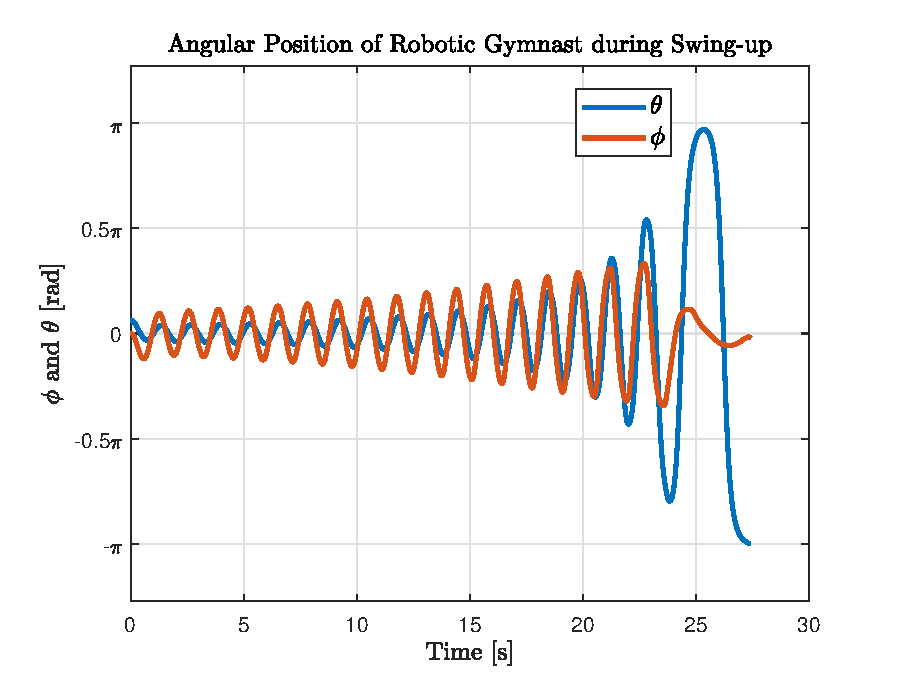
\includegraphics[scale=1]{./figs/swingup}
	\caption{Swing-up of the Robotic Gymnast}
	\label{fig:swingup}
\end{figure}

Figure \ref{fig:swingup} shows the swing-up controller swinging the robotic gymnast from it's stable equilibrium position to the vicinity of the unstable equilibrium position. There are a few interesting occurrences in the responses that were mentioned in the previous section to bring the reader's attention. Firstly the robotic gymnast is required to start at an initial condition for the swing-up control law to be active and this is seen with $\theta$ starting 11\textdegree. Secondly the amplitude of $\phi$ is seen to suddenly decrease when the system nears the inverted position. This is due to the $\alpha$ being reduced for reasons discussed.\\

The response shows the swing-up controller meets the designed requirements by swinging the robotic gymnast to the vicinity of the unstable equilibrium within 30 seconds and $\theta$ and $\phi$ is in the designed region for the balancing controller to bring the system to the inverted position.



\section{Simulation Results}
\begin{figure}[h]
	\centering
	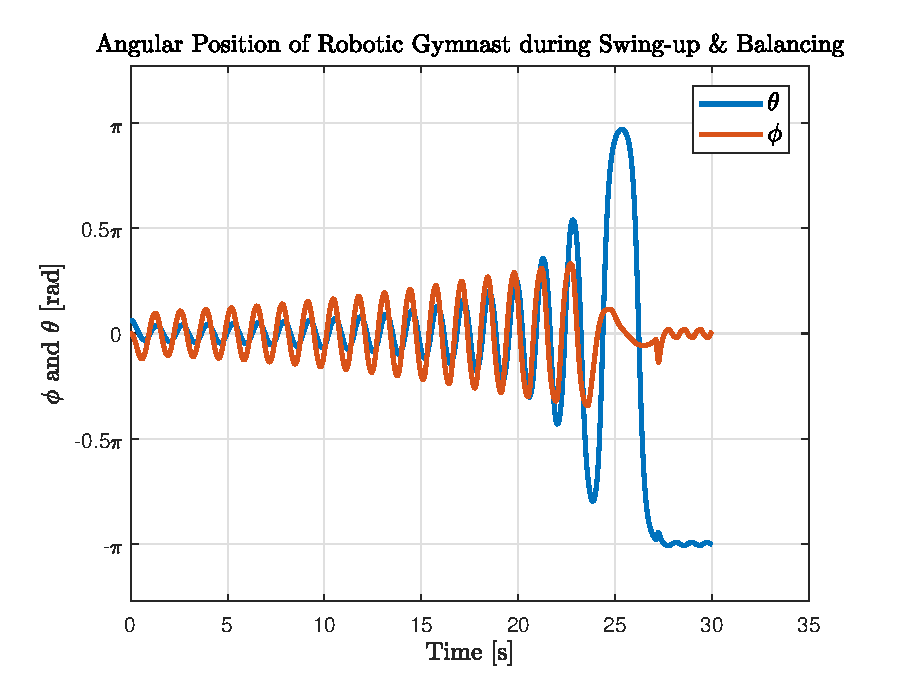
\includegraphics[scale=1]{./figs/swingup_balance}
	\caption{The Swing-Up \& Balancing of the Robotic Gymnast}
	\label{fig:swingup_balance}
\end{figure}